\documentclass[1p]{elsarticle_modified}
%\bibliographystyle{elsarticle-num}

%\usepackage[colorlinks]{hyperref}
%\usepackage{abbrmath_seonhwa} %\Abb, \Ascr, \Acal ,\Abf, \Afrak
\usepackage{amsfonts}
\usepackage{amssymb}
\usepackage{amsmath}
\usepackage{amsthm}
\usepackage{scalefnt}
\usepackage{amsbsy}
\usepackage{kotex}
\usepackage{caption}
\usepackage{subfig}
\usepackage{color}
\usepackage{graphicx}
\usepackage{xcolor} %% white, black, red, green, blue, cyan, magenta, yellow
\usepackage{float}
\usepackage{setspace}
\usepackage{hyperref}

\usepackage{tikz}
\usetikzlibrary{arrows}

\usepackage{multirow}
\usepackage{array} % fixed length table
\usepackage{hhline}

%%%%%%%%%%%%%%%%%%%%%
\makeatletter
\renewcommand*\env@matrix[1][\arraystretch]{%
	\edef\arraystretch{#1}%
	\hskip -\arraycolsep
	\let\@ifnextchar\new@ifnextchar
	\array{*\c@MaxMatrixCols c}}
\makeatother %https://tex.stackexchange.com/questions/14071/how-can-i-increase-the-line-spacing-in-a-matrix
%%%%%%%%%%%%%%%

\usepackage[normalem]{ulem}

\newcommand{\msout}[1]{\ifmmode\text{\sout{\ensuremath{#1}}}\else\sout{#1}\fi}
%SOURCE: \msout is \stkout macro in https://tex.stackexchange.com/questions/20609/strikeout-in-math-mode

\newcommand{\cancel}[1]{
	\ifmmode
	{\color{red}\msout{#1}}
	\else
	{\color{red}\sout{#1}}
	\fi
}

\newcommand{\add}[1]{
	{\color{blue}\uwave{#1}}
}

\newcommand{\replace}[2]{
	\ifmmode
	{\color{red}\msout{#1}}{\color{blue}\uwave{#2}}
	\else
	{\color{red}\sout{#1}}{\color{blue}\uwave{#2}}
	\fi
}

\newcommand{\Sol}{\mathcal{S}} %segment
\newcommand{\D}{D} %diagram
\newcommand{\A}{\mathcal{A}} %arc


%%%%%%%%%%%%%%%%%%%%%%%%%%%%%5 test

\def\sl{\operatorname{\textup{SL}}(2,\Cbb)}
\def\psl{\operatorname{\textup{PSL}}(2,\Cbb)}
\def\quan{\mkern 1mu \triangleright \mkern 1mu}

\theoremstyle{definition}
\newtheorem{thm}{Theorem}[section]
\newtheorem{prop}[thm]{Proposition}
\newtheorem{lem}[thm]{Lemma}
\newtheorem{ques}[thm]{Question}
\newtheorem{cor}[thm]{Corollary}
\newtheorem{defn}[thm]{Definition}
\newtheorem{exam}[thm]{Example}
\newtheorem{rmk}[thm]{Remark}
\newtheorem{alg}[thm]{Algorithm}

\newcommand{\I}{\sqrt{-1}}
\begin{document}

%\begin{frontmatter}
%
%\title{Boundary parabolic representations of knots up to 8 crossings}
%
%%% Group authors per affiliation:
%\author{Yunhi Cho} 
%\address{Department of Mathematics, University of Seoul, Seoul, Korea}
%\ead{yhcho@uos.ac.kr}
%
%
%\author{Seonhwa Kim} %\fnref{s_kim}}
%\address{Center for Geometry and Physics, Institute for Basic Science, Pohang, 37673, Korea}
%\ead{ryeona17@ibs.re.kr}
%
%\author{Hyuk Kim}
%\address{Department of Mathematical Sciences, Seoul National University, Seoul 08826, Korea}
%\ead{hyukkim@snu.ac.kr}
%
%\author{Seokbeom Yoon}
%\address{Department of Mathematical Sciences, Seoul National University, Seoul, 08826,  Korea}
%\ead{sbyoon15@snu.ac.kr}
%
%\begin{abstract}
%We find all boundary parabolic representation of knots up to 8 crossings.
%
%\end{abstract}
%\begin{keyword}
%    \MSC[2010] 57M25 
%\end{keyword}
%
%\end{frontmatter}

%\linenumbers
%\tableofcontents
%
\newcommand\colored[1]{\textcolor{white}{\rule[-0.35ex]{0.8em}{1.4ex}}\kern-0.8em\color{red} #1}%
%\newcommand\colored[1]{\textcolor{white}{ #1}\kern-2.17ex	\textcolor{white}{ #1}\kern-1.81ex	\textcolor{white}{ #1}\kern-2.15ex\color{red}#1	}

{\Large $\underline{12n_{0798}~(K12n_{0798})}$}

\setlength{\tabcolsep}{10pt}
\renewcommand{\arraystretch}{1.6}
\vspace{1cm}\begin{tabular}{m{100pt}>{\centering\arraybackslash}m{274pt}}
\multirow{5}{120pt}{
	\centering
	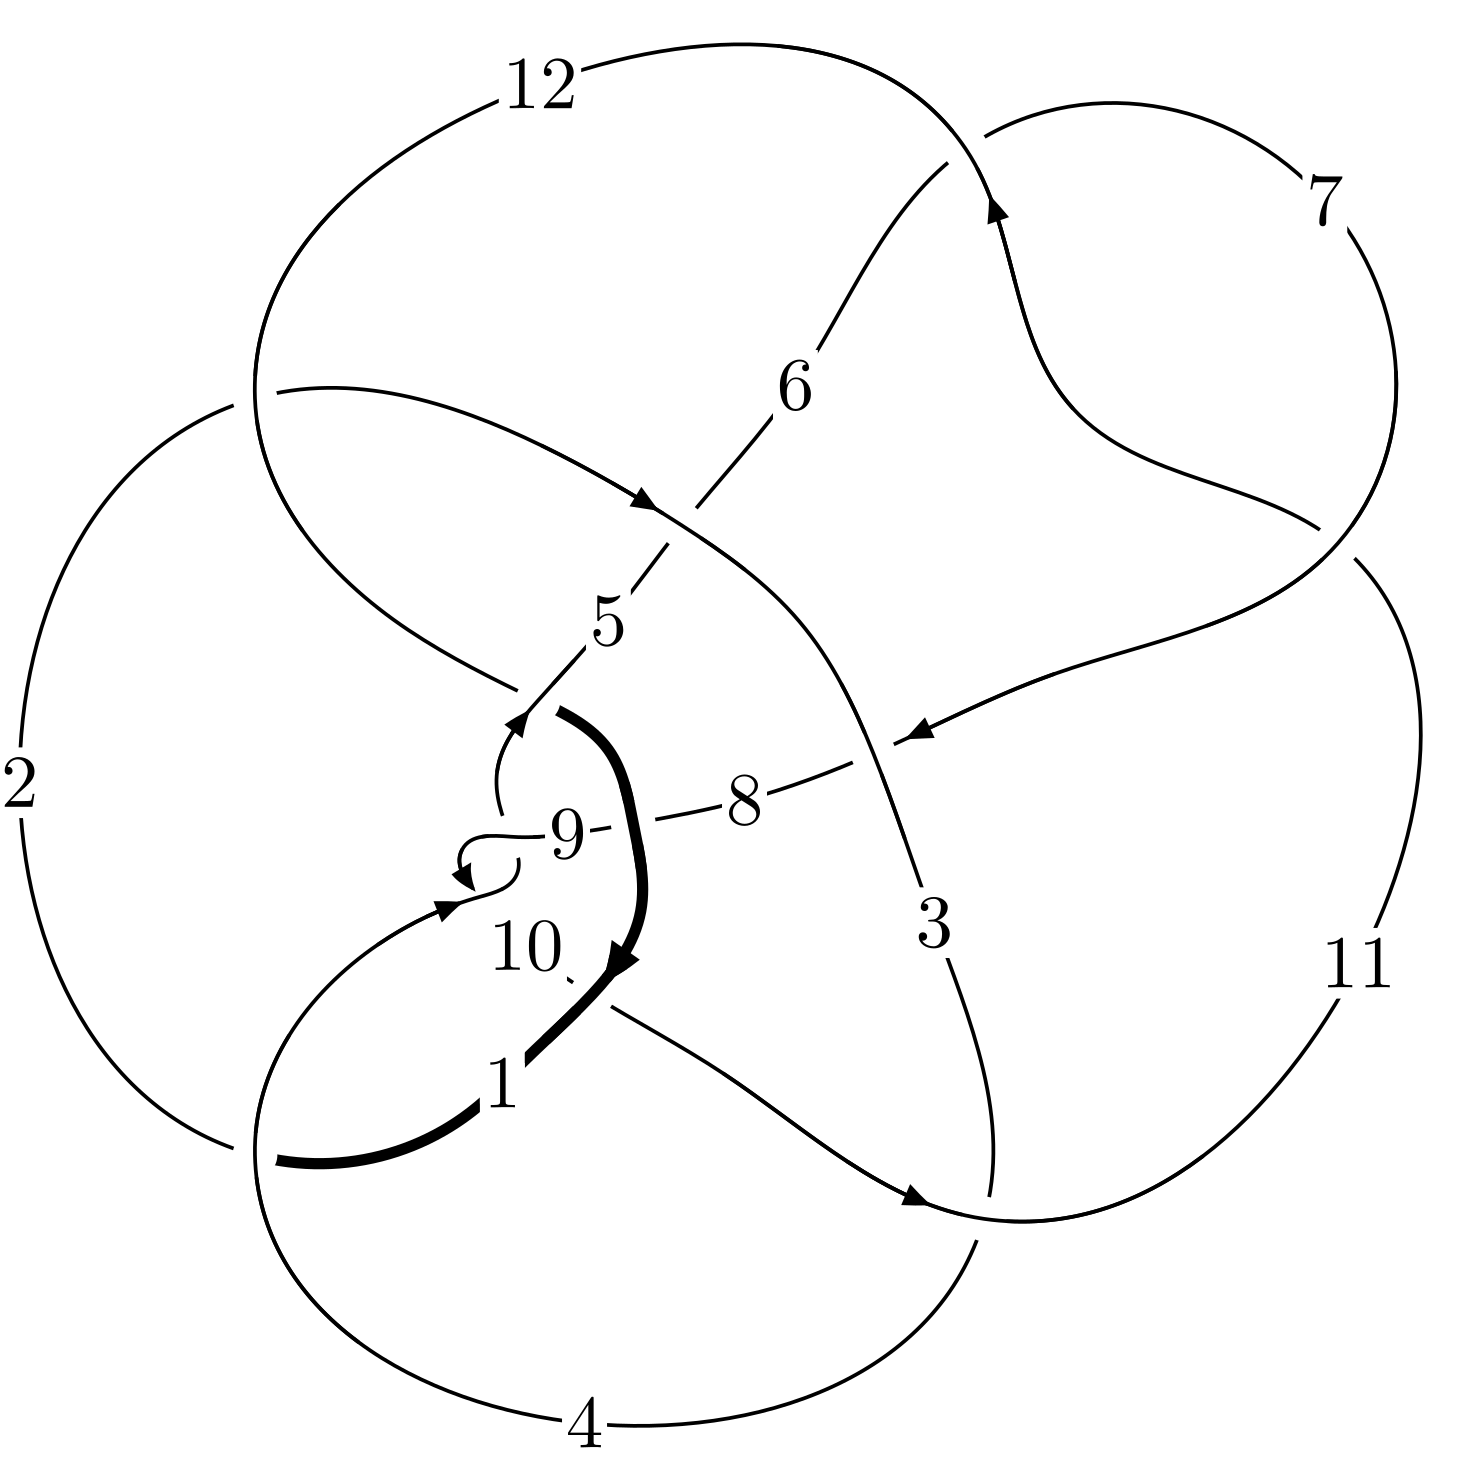
\includegraphics[width=112pt]{../../../GIT/diagram.site/Diagrams/png/2887_12n_0798.png}\\
\ \ \ A knot diagram\footnotemark}&
\allowdisplaybreaks
\textbf{Linearized knot diagam} \\
\cline{2-2}
 &
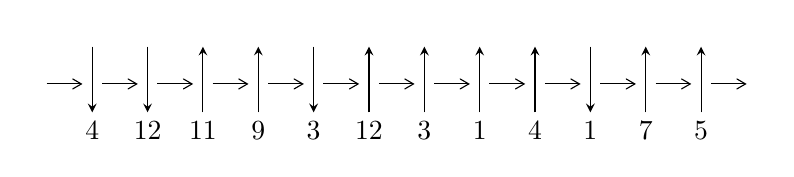
\begin{tikzpicture}[x=20pt, y=17pt]
	% nodes
	\node (C0) at (0, 0) {};
	\node (C1) at (1, 0) {};
	\node (C1U) at (1, +1) {};
	\node (C1D) at (1, -1) {4};

	\node (C2) at (2, 0) {};
	\node (C2U) at (2, +1) {};
	\node (C2D) at (2, -1) {12};

	\node (C3) at (3, 0) {};
	\node (C3U) at (3, +1) {};
	\node (C3D) at (3, -1) {11};

	\node (C4) at (4, 0) {};
	\node (C4U) at (4, +1) {};
	\node (C4D) at (4, -1) {9};

	\node (C5) at (5, 0) {};
	\node (C5U) at (5, +1) {};
	\node (C5D) at (5, -1) {3};

	\node (C6) at (6, 0) {};
	\node (C6U) at (6, +1) {};
	\node (C6D) at (6, -1) {12};

	\node (C7) at (7, 0) {};
	\node (C7U) at (7, +1) {};
	\node (C7D) at (7, -1) {3};

	\node (C8) at (8, 0) {};
	\node (C8U) at (8, +1) {};
	\node (C8D) at (8, -1) {1};

	\node (C9) at (9, 0) {};
	\node (C9U) at (9, +1) {};
	\node (C9D) at (9, -1) {4};

	\node (C10) at (10, 0) {};
	\node (C10U) at (10, +1) {};
	\node (C10D) at (10, -1) {1};

	\node (C11) at (11, 0) {};
	\node (C11U) at (11, +1) {};
	\node (C11D) at (11, -1) {7};

	\node (C12) at (12, 0) {};
	\node (C12U) at (12, +1) {};
	\node (C12D) at (12, -1) {5};
	\node (C13) at (13, 0) {};

	% arrows
	\draw[->,>={angle 60}]
	(C0) edge (C1) (C1) edge (C2) (C2) edge (C3) (C3) edge (C4) (C4) edge (C5) (C5) edge (C6) (C6) edge (C7) (C7) edge (C8) (C8) edge (C9) (C9) edge (C10) (C10) edge (C11) (C11) edge (C12) (C12) edge (C13) ;	\draw[->,>=stealth]
	(C1U) edge (C1D) (C2U) edge (C2D) (C3D) edge (C3U) (C4D) edge (C4U) (C5U) edge (C5D) (C6D) edge (C6U) (C7D) edge (C7U) (C8D) edge (C8U) (C9D) edge (C9U) (C10U) edge (C10D) (C11D) edge (C11U) (C12D) edge (C12U) ;
	\end{tikzpicture} \\
\hhline{~~} \\& 
\textbf{Solving Sequence} \\ \cline{2-2} 
 &
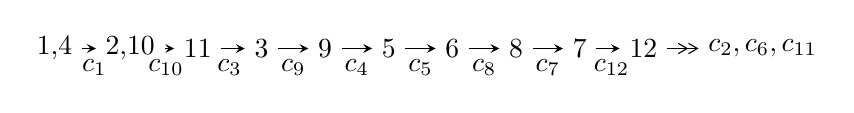
\begin{tikzpicture}[x=23pt, y=7pt]
	% node
	\node (A0) at (-1/8, 0) {1,4};
	\node (A1) at (17/16, 0) {2,10};
	\node (A2) at (17/8, 0) {11};
	\node (A3) at (25/8, 0) {3};
	\node (A4) at (33/8, 0) {9};
	\node (A5) at (41/8, 0) {5};
	\node (A6) at (49/8, 0) {6};
	\node (A7) at (57/8, 0) {8};
	\node (A8) at (65/8, 0) {7};
	\node (A9) at (73/8, 0) {12};
	\node (C1) at (1/2, -1) {$c_{1}$};
	\node (C2) at (13/8, -1) {$c_{10}$};
	\node (C3) at (21/8, -1) {$c_{3}$};
	\node (C4) at (29/8, -1) {$c_{9}$};
	\node (C5) at (37/8, -1) {$c_{4}$};
	\node (C6) at (45/8, -1) {$c_{5}$};
	\node (C7) at (53/8, -1) {$c_{8}$};
	\node (C8) at (61/8, -1) {$c_{7}$};
	\node (C9) at (69/8, -1) {$c_{12}$};
	\node (A10) at (11, 0) {$c_{2},c_{6},c_{11}$};

	% edge
	\draw[->,>=stealth]	
	(A0) edge (A1) (A1) edge (A2) (A2) edge (A3) (A3) edge (A4) (A4) edge (A5) (A5) edge (A6) (A6) edge (A7) (A7) edge (A8) (A8) edge (A9) ;
	\draw[->>,>={angle 60}]	
	(A9) edge (A10);
\end{tikzpicture} \\ 

\end{tabular} \\

\footnotetext{
The image of knot diagram is generated by the software ``\textbf{Draw programme}" developed by Andrew Bartholomew(\url{http://www.layer8.co.uk/maths/draw/index.htm\#Running-draw}), where we modified some parts for our purpose(\url{https://github.com/CATsTAILs/LinksPainter}).
}\phantom \\ \newline 
\centering \textbf{Ideals for irreducible components\footnotemark of $X_{\text{par}}$} 
 
\begin{align*}
I^u_{1}&=\langle 
1283 u^{12}-662 u^{11}+\cdots+5739 b+1160,\;-630 u^{12}+3164 u^{11}+\cdots+1913 a-753,\\
\phantom{I^u_{1}}&\phantom{= \langle  }u^{13}-3 u^{12}+8 u^{11}-20 u^{10}+36 u^9-61 u^8+84 u^7-97 u^6+97 u^5-68 u^4+41 u^3-13 u^2+3 u+1\rangle \\
I^u_{2}&=\langle 
-1.18123\times10^{153} u^{55}-4.51937\times10^{153} u^{54}+\cdots+2.08930\times10^{155} b-7.05789\times10^{155},\\
\phantom{I^u_{2}}&\phantom{= \langle  }8.87232\times10^{153} u^{55}+3.38341\times10^{154} u^{54}+\cdots+6.26789\times10^{155} a+3.97690\times10^{156},\\
\phantom{I^u_{2}}&\phantom{= \langle  }u^{56}+4 u^{55}+\cdots+1346 u+111\rangle \\
I^u_{3}&=\langle 
-135214 u^{15}+515373 u^{14}+\cdots+267063 b+30946,\\
\phantom{I^u_{3}}&\phantom{= \langle  }-570167 u^{15}+1972254 u^{14}+\cdots+1335315 a-4248919,\;u^{16}-4 u^{15}+\cdots- u+1\rangle \\
I^u_{4}&=\langle 
- u^3+u^2+b- u,\;u^2+a- u+2,\;u^4- u^3+2 u^2+1\rangle \\
I^u_{5}&=\langle 
- u^2+b+u,\;a+u,\;u^4- u^3+u^2- u+1\rangle \\
\\
\end{align*}
\raggedright * 5 irreducible components of $\dim_{\mathbb{C}}=0$, with total 93 representations.\\
\footnotetext{All coefficients of polynomials are rational numbers. But the coefficients are sometimes approximated in decimal forms when there is not enough margin.}
\newpage
\renewcommand{\arraystretch}{1}
\centering \section*{I. $I^u_{1}= \langle 1283 u^{12}-662 u^{11}+\cdots+5739 b+1160,\;-630 u^{12}+3164 u^{11}+\cdots+1913 a-753,\;u^{13}-3 u^{12}+\cdots+3 u+1 \rangle$}
\flushleft \textbf{(i) Arc colorings}\\
\begin{tabular}{m{7pt} m{180pt} m{7pt} m{180pt} }
\flushright $a_{1}=$&$\begin{pmatrix}1\\0\end{pmatrix}$ \\
\flushright $a_{4}=$&$\begin{pmatrix}0\\u\end{pmatrix}$ \\
\flushright $a_{2}=$&$\begin{pmatrix}1\\u^2\end{pmatrix}$ \\
\flushright $a_{10}=$&$\begin{pmatrix}0.329326 u^{12}-1.65395 u^{11}+\cdots-12.3325 u+0.393623\\-0.223558 u^{12}+0.115351 u^{11}+\cdots-2.77749 u-0.202126\end{pmatrix}$ \\
\flushright $a_{11}=$&$\begin{pmatrix}0.552884 u^{12}-1.76930 u^{11}+\cdots-9.55497 u+0.595748\\-0.223558 u^{12}+0.115351 u^{11}+\cdots-2.77749 u-0.202126\end{pmatrix}$ \\
\flushright $a_{3}=$&$\begin{pmatrix}-0.744555 u^{12}+1.43562 u^{11}+\cdots-4.66423 u+0.635477\\-0.238021 u^{12}+0.958355 u^{11}+\cdots+3.13870 u+0.798048\end{pmatrix}$ \\
\flushright $a_{9}=$&$\begin{pmatrix}0.329326 u^{12}-1.65395 u^{11}+\cdots-12.3325 u+0.393623\\-0.499042 u^{12}+1.07667 u^{11}+\cdots-1.10890 u+0.463844\end{pmatrix}$ \\
\flushright $a_{5}=$&$\begin{pmatrix}1.02248 u^{12}-2.20178 u^{11}+\cdots+4.08207 u-1.12075\\-0.110646 u^{12}+0.148284 u^{11}+\cdots-1.06290 u-0.552884\end{pmatrix}$ \\
\flushright $a_{6}=$&$\begin{pmatrix}0.905558 u^{12}-2.55532 u^{11}+\cdots-1.63164 u-1.70971\\-0.659697 u^{12}+2.22426 u^{11}+\cdots+3.05646 u+0.706743\end{pmatrix}$ \\
\flushright $a_{8}=$&$\begin{pmatrix}0.828367 u^{12}-2.73062 u^{11}+\cdots-11.2236 u-0.0702213\\-0.499042 u^{12}+1.07667 u^{11}+\cdots-1.10890 u+0.463844\end{pmatrix}$ \\
\flushright $a_{7}=$&$\begin{pmatrix}1.44642 u^{12}-3.28646 u^{11}+\cdots-1.18400 u+1.06691\\0.158564 u^{12}-1.31486 u^{11}+\cdots-7.38230 u-1.25492\end{pmatrix}$ \\
\flushright $a_{12}=$&$\begin{pmatrix}-0.364523 u^{12}+1.83813 u^{11}+\cdots+7.51403 u+3.57066\\0.798048 u^{12}-2.15612 u^{11}+\cdots-2.86914 u-0.744555\end{pmatrix}$\\&\end{tabular}
\flushleft \textbf{(ii) Obstruction class $= -1$}\\~\\
\flushleft \textbf{(iii) Cusp Shapes $= \frac{27061}{5739} u^{12}-\frac{84808}{5739} u^{11}+\cdots-\frac{197266}{5739} u+\frac{6865}{5739}$}\\~\\
\newpage\renewcommand{\arraystretch}{1}
\flushleft \textbf{(iv) u-Polynomials at the component}\newline \\
\begin{tabular}{m{50pt}|m{274pt}}
Crossings & \hspace{64pt}u-Polynomials at each crossing \\
\hline $$\begin{aligned}c_{1},c_{2}\end{aligned}$$&$\begin{aligned}
&u^{13}+3 u^{12}+\cdots+3 u-1
\end{aligned}$\\
\hline $$\begin{aligned}c_{3},c_{12}\end{aligned}$$&$\begin{aligned}
&u^{13}+u^{12}+\cdots-3 u-1
\end{aligned}$\\
\hline $$\begin{aligned}c_{4},c_{6},c_{9}\\c_{11}\end{aligned}$$&$\begin{aligned}
&u^{13}-2 u^{12}+\cdots+7 u^3-1
\end{aligned}$\\
\hline $$\begin{aligned}c_{5},c_{10}\end{aligned}$$&$\begin{aligned}
&u^{13}- u^{12}+\cdots+3 u-3
\end{aligned}$\\
\hline $$\begin{aligned}c_{7},c_{8}\end{aligned}$$&$\begin{aligned}
&u^{13}+3 u^{12}+\cdots-8 u-3
\end{aligned}$\\
\hline
\end{tabular}\\~\\
\newpage\renewcommand{\arraystretch}{1}
\flushleft \textbf{(v) Riley Polynomials at the component}\newline \\
\begin{tabular}{m{50pt}|m{274pt}}
Crossings & \hspace{64pt}Riley Polynomials at each crossing \\
\hline $$\begin{aligned}c_{1},c_{2}\end{aligned}$$&$\begin{aligned}
&y^{13}+7 y^{12}+\cdots+35 y-1
\end{aligned}$\\
\hline $$\begin{aligned}c_{3},c_{12}\end{aligned}$$&$\begin{aligned}
&y^{13}+7 y^{12}+\cdots+3 y-1
\end{aligned}$\\
\hline $$\begin{aligned}c_{4},c_{6},c_{9}\\c_{11}\end{aligned}$$&$\begin{aligned}
&y^{13}+4 y^{11}+\cdots-2 y^2-1
\end{aligned}$\\
\hline $$\begin{aligned}c_{5},c_{10}\end{aligned}$$&$\begin{aligned}
&y^{13}+15 y^{12}+\cdots+39 y-9
\end{aligned}$\\
\hline $$\begin{aligned}c_{7},c_{8}\end{aligned}$$&$\begin{aligned}
&y^{13}-3 y^{12}+\cdots+34 y-9
\end{aligned}$\\
\hline
\end{tabular}\\~\\
\newpage\flushleft \textbf{(vi) Complex Volumes and Cusp Shapes}
$$\begin{array}{c|c|c}  
\text{Solutions to }I^u_{1}& \I (\text{vol} + \sqrt{-1}CS) & \text{Cusp shape}\\
 \hline 
\begin{aligned}
u &= \phantom{-}0.125889 + 0.791075 I \\
a &= -0.42819 + 1.60424 I \\
b &= \phantom{-}0.06421 + 1.99251 I\end{aligned}
 & \phantom{-}3.78832 - 0.68098 I & \phantom{-}3.18600 + 10.56387 I \\ \hline\begin{aligned}
u &= \phantom{-}0.125889 - 0.791075 I \\
a &= -0.42819 - 1.60424 I \\
b &= \phantom{-}0.06421 - 1.99251 I\end{aligned}
 & \phantom{-}3.78832 + 0.68098 I & \phantom{-}3.18600 - 10.56387 I \\ \hline\begin{aligned}
u &= \phantom{-}0.435895 + 1.153550 I \\
a &= -0.166988 - 0.397762 I \\
b &= -1.101790 - 0.664354 I\end{aligned}
 & -1.60930 - 2.98509 I & \phantom{-}6.45992 + 2.62910 I \\ \hline\begin{aligned}
u &= \phantom{-}0.435895 - 1.153550 I \\
a &= -0.166988 + 0.397762 I \\
b &= -1.101790 + 0.664354 I\end{aligned}
 & -1.60930 + 2.98509 I & \phantom{-}6.45992 - 2.62910 I \\ \hline\begin{aligned}
u &= \phantom{-}0.405751 + 0.538490 I \\
a &= -1.29934 - 1.45999 I \\
b &= \phantom{-}0.613689 - 0.351552 I\end{aligned}
 & -8.20006 - 2.65719 I & -7.53293 + 6.11651 I \\ \hline\begin{aligned}
u &= \phantom{-}0.405751 - 0.538490 I \\
a &= -1.29934 + 1.45999 I \\
b &= \phantom{-}0.613689 + 0.351552 I\end{aligned}
 & -8.20006 + 2.65719 I & -7.53293 - 6.11651 I \\ \hline\begin{aligned}
u &= -0.21582 + 1.42915 I \\
a &= \phantom{-}0.743610 + 0.701361 I \\
b &= \phantom{-}0.17608 + 1.54701 I\end{aligned}
 & \phantom{-}9.07015 + 0.94105 I & \phantom{-}7.27747 - 1.09961 I \\ \hline\begin{aligned}
u &= -0.21582 - 1.42915 I \\
a &= \phantom{-}0.743610 - 0.701361 I \\
b &= \phantom{-}0.17608 - 1.54701 I\end{aligned}
 & \phantom{-}9.07015 - 0.94105 I & \phantom{-}7.27747 + 1.09961 I \\ \hline\begin{aligned}
u &= \phantom{-}1.52678 + 0.05294 I \\
a &= \phantom{-}0.101352 + 0.424061 I \\
b &= -0.310928 + 0.347924 I\end{aligned}
 & -3.37050 + 0.66803 I & \phantom{-}1.81891 - 10.95758 I \\ \hline\begin{aligned}
u &= \phantom{-}1.52678 - 0.05294 I \\
a &= \phantom{-}0.101352 - 0.424061 I \\
b &= -0.310928 - 0.347924 I\end{aligned}
 & -3.37050 - 0.66803 I & \phantom{-}1.81891 + 10.95758 I\\
 \hline 
 \end{array}$$\newpage$$\begin{array}{c|c|c}  
\text{Solutions to }I^u_{1}& \I (\text{vol} + \sqrt{-1}CS) & \text{Cusp shape}\\
 \hline 
\begin{aligned}
u &= -0.70010 + 1.56807 I \\
a &= \phantom{-}0.383909 - 0.789778 I \\
b &= \phantom{-}0.82111 - 1.72051 I\end{aligned}
 & \phantom{-}7.2980 + 16.4758 I & \phantom{-}4.42093 - 8.40539 I \\ \hline\begin{aligned}
u &= -0.70010 - 1.56807 I \\
a &= \phantom{-}0.383909 + 0.789778 I \\
b &= \phantom{-}0.82111 + 1.72051 I\end{aligned}
 & \phantom{-}7.2980 - 16.4758 I & \phantom{-}4.42093 + 8.40539 I \\ \hline\begin{aligned}
u &= -0.156796\phantom{ +0.000000I} \\
a &= \phantom{-}3.33128\phantom{ +0.000000I} \\
b &= \phantom{-}0.475252\phantom{ +0.000000I}\end{aligned}
 & \phantom{-}0.851273\phantom{ +0.000000I} & \phantom{-}11.7390\phantom{ +0.000000I}\\
 \hline 
 \end{array}$$\newpage\newpage\renewcommand{\arraystretch}{1}
\centering \section*{II. $I^u_{2}= \langle -1.18\times10^{153} u^{55}-4.52\times10^{153} u^{54}+\cdots+2.09\times10^{155} b-7.06\times10^{155},\;8.87\times10^{153} u^{55}+3.38\times10^{154} u^{54}+\cdots+6.27\times10^{155} a+3.98\times10^{156},\;u^{56}+4 u^{55}+\cdots+1346 u+111 \rangle$}
\flushleft \textbf{(i) Arc colorings}\\
\begin{tabular}{m{7pt} m{180pt} m{7pt} m{180pt} }
\flushright $a_{1}=$&$\begin{pmatrix}1\\0\end{pmatrix}$ \\
\flushright $a_{4}=$&$\begin{pmatrix}0\\u\end{pmatrix}$ \\
\flushright $a_{2}=$&$\begin{pmatrix}1\\u^2\end{pmatrix}$ \\
\flushright $a_{10}=$&$\begin{pmatrix}-0.0141552 u^{55}-0.0539800 u^{54}+\cdots-28.3025 u-6.34487\\0.00565370 u^{55}+0.0216310 u^{54}+\cdots+16.5561 u+3.37812\end{pmatrix}$ \\
\flushright $a_{11}=$&$\begin{pmatrix}-0.0198089 u^{55}-0.0756110 u^{54}+\cdots-44.8585 u-9.72299\\0.00565370 u^{55}+0.0216310 u^{54}+\cdots+16.5561 u+3.37812\end{pmatrix}$ \\
\flushright $a_{3}=$&$\begin{pmatrix}0.0144678 u^{55}+0.0586721 u^{54}+\cdots+73.1975 u+12.4499\\-0.00267933 u^{55}-0.00908580 u^{54}+\cdots-12.7090 u-3.57215\end{pmatrix}$ \\
\flushright $a_{9}=$&$\begin{pmatrix}-0.0141552 u^{55}-0.0539800 u^{54}+\cdots-28.3025 u-6.34487\\0.00718179 u^{55}+0.0273575 u^{54}+\cdots+14.5728 u+3.08499\end{pmatrix}$ \\
\flushright $a_{5}=$&$\begin{pmatrix}-0.00877254 u^{55}-0.0387439 u^{54}+\cdots-48.2032 u-6.38465\\0.00314979 u^{55}+0.0134163 u^{54}+\cdots+18.1770 u+2.89867\end{pmatrix}$ \\
\flushright $a_{6}=$&$\begin{pmatrix}-0.0116448 u^{55}-0.0480523 u^{54}+\cdots-48.8452 u+1.49968\\0.00331140 u^{55}+0.0134797 u^{54}+\cdots+33.1904 u+2.23101\end{pmatrix}$ \\
\flushright $a_{8}=$&$\begin{pmatrix}-0.0213370 u^{55}-0.0813374 u^{54}+\cdots-42.8753 u-9.42987\\0.00718179 u^{55}+0.0273575 u^{54}+\cdots+14.5728 u+3.08499\end{pmatrix}$ \\
\flushright $a_{7}=$&$\begin{pmatrix}0.0106076 u^{55}+0.0439229 u^{54}+\cdots+51.7711 u+2.93855\\-0.00286600 u^{55}-0.0111012 u^{54}+\cdots-25.2269 u-2.36948\end{pmatrix}$ \\
\flushright $a_{12}=$&$\begin{pmatrix}-0.00420227 u^{55}-0.0147886 u^{54}+\cdots-32.7418 u-2.34305\\0.00309502 u^{55}+0.0110761 u^{54}+\cdots+17.1401 u+2.03269\end{pmatrix}$\\&\end{tabular}
\flushleft \textbf{(ii) Obstruction class $= -1$}\\~\\
\flushleft \textbf{(iii) Cusp Shapes $= -0.000431876 u^{55}-0.00131056 u^{54}+\cdots-42.1688 u+5.52954$}\\~\\
\newpage\renewcommand{\arraystretch}{1}
\flushleft \textbf{(iv) u-Polynomials at the component}\newline \\
\begin{tabular}{m{50pt}|m{274pt}}
Crossings & \hspace{64pt}u-Polynomials at each crossing \\
\hline $$\begin{aligned}c_{1},c_{2}\end{aligned}$$&$\begin{aligned}
&u^{56}-4 u^{55}+\cdots-1346 u+111
\end{aligned}$\\
\hline $$\begin{aligned}c_{3},c_{12}\end{aligned}$$&$\begin{aligned}
&u^{56}+2 u^{54}+\cdots+907 u+193
\end{aligned}$\\
\hline $$\begin{aligned}c_{4},c_{6},c_{9}\\c_{11}\end{aligned}$$&$\begin{aligned}
&u^{56}+u^{55}+\cdots+13 u+3
\end{aligned}$\\
\hline $$\begin{aligned}c_{5},c_{10}\end{aligned}$$&$\begin{aligned}
&u^{56}+2 u^{55}+\cdots+82 u+37
\end{aligned}$\\
\hline $$\begin{aligned}c_{7},c_{8}\end{aligned}$$&$\begin{aligned}
&u^{56}- u^{55}+\cdots+29361 u+1951
\end{aligned}$\\
\hline
\end{tabular}\\~\\
\newpage\renewcommand{\arraystretch}{1}
\flushleft \textbf{(v) Riley Polynomials at the component}\newline \\
\begin{tabular}{m{50pt}|m{274pt}}
Crossings & \hspace{64pt}Riley Polynomials at each crossing \\
\hline $$\begin{aligned}c_{1},c_{2}\end{aligned}$$&$\begin{aligned}
&y^{56}+50 y^{55}+\cdots-249724 y+12321
\end{aligned}$\\
\hline $$\begin{aligned}c_{3},c_{12}\end{aligned}$$&$\begin{aligned}
&y^{56}+4 y^{55}+\cdots-242491 y+37249
\end{aligned}$\\
\hline $$\begin{aligned}c_{4},c_{6},c_{9}\\c_{11}\end{aligned}$$&$\begin{aligned}
&y^{56}+15 y^{55}+\cdots+275 y+9
\end{aligned}$\\
\hline $$\begin{aligned}c_{5},c_{10}\end{aligned}$$&$\begin{aligned}
&y^{56}+52 y^{55}+\cdots-39284 y+1369
\end{aligned}$\\
\hline $$\begin{aligned}c_{7},c_{8}\end{aligned}$$&$\begin{aligned}
&y^{56}-31 y^{55}+\cdots-114413905 y+3806401
\end{aligned}$\\
\hline
\end{tabular}\\~\\
\newpage\flushleft \textbf{(vi) Complex Volumes and Cusp Shapes}
$$\begin{array}{c|c|c}  
\text{Solutions to }I^u_{2}& \I (\text{vol} + \sqrt{-1}CS) & \text{Cusp shape}\\
 \hline 
\begin{aligned}
u &= \phantom{-}0.973175 + 0.358698 I \\
a &= \phantom{-}0.223686 + 0.715699 I \\
b &= -0.141495 - 0.212809 I\end{aligned}
 & -2.35105 - 1.37665 I & \phantom{-0.000000 -}0. + 4.49216 I \\ \hline\begin{aligned}
u &= \phantom{-}0.973175 - 0.358698 I \\
a &= \phantom{-}0.223686 - 0.715699 I \\
b &= -0.141495 + 0.212809 I\end{aligned}
 & -2.35105 + 1.37665 I & \phantom{-0.000000 } 0. - 4.49216 I \\ \hline\begin{aligned}
u &= -0.847096 + 0.638226 I \\
a &= -0.404462 + 0.469747 I \\
b &= \phantom{-}0.15766 + 1.46714 I\end{aligned}
 & \phantom{-}1.93596 + 5.90600 I & \phantom{-0.000000 } 0. - 3.51945 I \\ \hline\begin{aligned}
u &= -0.847096 - 0.638226 I \\
a &= -0.404462 - 0.469747 I \\
b &= \phantom{-}0.15766 - 1.46714 I\end{aligned}
 & \phantom{-}1.93596 - 5.90600 I & \phantom{-0.000000 -}0. + 3.51945 I \\ \hline\begin{aligned}
u &= -0.561985 + 0.926870 I \\
a &= \phantom{-}0.331742 - 1.143620 I \\
b &= \phantom{-}0.25987 - 1.69030 I\end{aligned}
 & -3.01211 + 5.08083 I & \phantom{-}8.72700 + 0. I\phantom{ +0.000000I} \\ \hline\begin{aligned}
u &= -0.561985 - 0.926870 I \\
a &= \phantom{-}0.331742 + 1.143620 I \\
b &= \phantom{-}0.25987 + 1.69030 I\end{aligned}
 & -3.01211 - 5.08083 I & \phantom{-}8.72700 + 0. I\phantom{ +0.000000I} \\ \hline\begin{aligned}
u &= -0.401455 + 0.819963 I \\
a &= \phantom{-}0.524050 - 0.252083 I \\
b &= -0.232565 - 1.287120 I\end{aligned}
 & \phantom{-}3.14992 - 0.89303 I & \phantom{-}3.36391 + 1.60851 I \\ \hline\begin{aligned}
u &= -0.401455 - 0.819963 I \\
a &= \phantom{-}0.524050 + 0.252083 I \\
b &= -0.232565 + 1.287120 I\end{aligned}
 & \phantom{-}3.14992 + 0.89303 I & \phantom{-}3.36391 - 1.60851 I \\ \hline\begin{aligned}
u &= \phantom{-}0.428842 + 0.782748 I \\
a &= \phantom{-}1.39747 + 0.43456 I \\
b &= -0.093467 - 0.473397 I\end{aligned}
 & -2.65912 - 0.69416 I & \phantom{-}5.49287 + 3.59719 I \\ \hline\begin{aligned}
u &= \phantom{-}0.428842 - 0.782748 I \\
a &= \phantom{-}1.39747 - 0.43456 I \\
b &= -0.093467 + 0.473397 I\end{aligned}
 & -2.65912 + 0.69416 I & \phantom{-}5.49287 - 3.59719 I\\
 \hline 
 \end{array}$$\newpage$$\begin{array}{c|c|c}  
\text{Solutions to }I^u_{2}& \I (\text{vol} + \sqrt{-1}CS) & \text{Cusp shape}\\
 \hline 
\begin{aligned}
u &= -0.293234 + 1.071580 I \\
a &= -0.398636 + 1.032790 I \\
b &= \phantom{-}0.105708 + 1.267210 I\end{aligned}
 & \phantom{-}3.14992 + 0.89303 I & \phantom{-}4.00000 + 0. I\phantom{ +0.000000I} \\ \hline\begin{aligned}
u &= -0.293234 - 1.071580 I \\
a &= -0.398636 - 1.032790 I \\
b &= \phantom{-}0.105708 - 1.267210 I\end{aligned}
 & \phantom{-}3.14992 - 0.89303 I & \phantom{-}4.00000 + 0. I\phantom{ +0.000000I} \\ \hline\begin{aligned}
u &= -0.087731 + 1.118910 I \\
a &= -0.686073 + 0.991907 I \\
b &= \phantom{-}0.06046 + 1.60533 I\end{aligned}
 & \phantom{-}3.57949 + 0.97368 I & \phantom{-}7.35348 - 5.23167 I \\ \hline\begin{aligned}
u &= -0.087731 - 1.118910 I \\
a &= -0.686073 - 0.991907 I \\
b &= \phantom{-}0.06046 - 1.60533 I\end{aligned}
 & \phantom{-}3.57949 - 0.97368 I & \phantom{-}7.35348 + 5.23167 I \\ \hline\begin{aligned}
u &= \phantom{-}0.683985 + 0.326867 I \\
a &= \phantom{-}0.76677 + 1.25863 I \\
b &= -0.876249 - 0.500129 I\end{aligned}
 & -4.38515 - 0.94897 I & -10.21959 + 1.75938 I \\ \hline\begin{aligned}
u &= \phantom{-}0.683985 - 0.326867 I \\
a &= \phantom{-}0.76677 - 1.25863 I \\
b &= -0.876249 + 0.500129 I\end{aligned}
 & -4.38515 + 0.94897 I & -10.21959 - 1.75938 I \\ \hline\begin{aligned}
u &= -0.463157 + 1.179820 I \\
a &= -0.692781 - 0.317187 I \\
b &= -0.447756 - 0.568276 I\end{aligned}
 & -2.65912 - 0.69416 I & \phantom{-0.000000 } 0 \\ \hline\begin{aligned}
u &= -0.463157 - 1.179820 I \\
a &= -0.692781 + 0.317187 I \\
b &= -0.447756 + 0.568276 I\end{aligned}
 & -2.65912 + 0.69416 I & \phantom{-0.000000 } 0 \\ \hline\begin{aligned}
u &= -1.250640 + 0.306528 I \\
a &= \phantom{-}0.350610 + 0.608692 I \\
b &= -0.076204 + 0.243308 I\end{aligned}
 & \phantom{-}3.22350 + 2.16516 I & \phantom{-0.000000 } 0 \\ \hline\begin{aligned}
u &= -1.250640 - 0.306528 I \\
a &= \phantom{-}0.350610 - 0.608692 I \\
b &= -0.076204 - 0.243308 I\end{aligned}
 & \phantom{-}3.22350 - 2.16516 I & \phantom{-0.000000 } 0\\
 \hline 
 \end{array}$$\newpage$$\begin{array}{c|c|c}  
\text{Solutions to }I^u_{2}& \I (\text{vol} + \sqrt{-1}CS) & \text{Cusp shape}\\
 \hline 
\begin{aligned}
u &= -0.150720 + 1.306260 I \\
a &= \phantom{-}0.728240 + 0.063856 I \\
b &= \phantom{-}1.105270 + 0.474638 I\end{aligned}
 & -0.60047 - 5.02443 I & \phantom{-0.000000 } 0 \\ \hline\begin{aligned}
u &= -0.150720 - 1.306260 I \\
a &= \phantom{-}0.728240 - 0.063856 I \\
b &= \phantom{-}1.105270 - 0.474638 I\end{aligned}
 & -0.60047 + 5.02443 I & \phantom{-0.000000 } 0 \\ \hline\begin{aligned}
u &= \phantom{-}0.118150 + 1.326950 I \\
a &= \phantom{-}0.824150 + 0.704249 I \\
b &= -0.25793 + 1.46755 I\end{aligned}
 & \phantom{-}7.25514\phantom{ +0.000000I} & \phantom{-0.000000 } 0 \\ \hline\begin{aligned}
u &= \phantom{-}0.118150 - 1.326950 I \\
a &= \phantom{-}0.824150 - 0.704249 I \\
b &= -0.25793 - 1.46755 I\end{aligned}
 & \phantom{-}7.25514\phantom{ +0.000000I} & \phantom{-0.000000 } 0 \\ \hline\begin{aligned}
u &= \phantom{-}0.855631 + 1.049130 I \\
a &= -0.036172 - 0.766616 I \\
b &= -0.62639 - 1.44617 I\end{aligned}
 & -0.60047 - 5.02443 I & \phantom{-0.000000 } 0 \\ \hline\begin{aligned}
u &= \phantom{-}0.855631 - 1.049130 I \\
a &= -0.036172 + 0.766616 I \\
b &= -0.62639 + 1.44617 I\end{aligned}
 & -0.60047 + 5.02443 I & \phantom{-0.000000 } 0 \\ \hline\begin{aligned}
u &= \phantom{-}0.110352 + 0.636373 I \\
a &= -2.55589 - 0.04098 I \\
b &= -0.423182 + 0.031837 I\end{aligned}
 & -3.01211 + 5.08083 I & \phantom{-}8.72700 - 0.16788 I \\ \hline\begin{aligned}
u &= \phantom{-}0.110352 - 0.636373 I \\
a &= -2.55589 + 0.04098 I \\
b &= -0.423182 - 0.031837 I\end{aligned}
 & -3.01211 - 5.08083 I & \phantom{-}8.72700 + 0.16788 I \\ \hline\begin{aligned}
u &= -0.002625 + 1.377270 I \\
a &= \phantom{-}0.508986 - 0.612116 I \\
b &= -0.09477 - 1.51750 I\end{aligned}
 & \phantom{-}3.22350 - 2.16516 I & \phantom{-0.000000 } 0 \\ \hline\begin{aligned}
u &= -0.002625 - 1.377270 I \\
a &= \phantom{-}0.508986 + 0.612116 I \\
b &= -0.09477 + 1.51750 I\end{aligned}
 & \phantom{-}3.22350 + 2.16516 I & \phantom{-0.000000 } 0\\
 \hline 
 \end{array}$$\newpage$$\begin{array}{c|c|c}  
\text{Solutions to }I^u_{2}& \I (\text{vol} + \sqrt{-1}CS) & \text{Cusp shape}\\
 \hline 
\begin{aligned}
u &= \phantom{-}0.150210 + 0.569344 I \\
a &= -0.824610 - 0.889775 I \\
b &= -1.046740 + 0.070502 I\end{aligned}
 & -2.35105 - 1.37665 I & -0.14056 + 4.49216 I \\ \hline\begin{aligned}
u &= \phantom{-}0.150210 - 0.569344 I \\
a &= -0.824610 + 0.889775 I \\
b &= -1.046740 - 0.070502 I\end{aligned}
 & -2.35105 + 1.37665 I & -0.14056 - 4.49216 I \\ \hline\begin{aligned}
u &= -0.23885 + 1.42021 I \\
a &= -0.724589 - 0.727418 I \\
b &= \phantom{-}0.07102 - 1.58823 I\end{aligned}
 & \phantom{-}8.32665 + 8.69653 I & \phantom{-0.000000 } 0 \\ \hline\begin{aligned}
u &= -0.23885 - 1.42021 I \\
a &= -0.724589 + 0.727418 I \\
b &= \phantom{-}0.07102 + 1.58823 I\end{aligned}
 & \phantom{-}8.32665 - 8.69653 I & \phantom{-0.000000 } 0 \\ \hline\begin{aligned}
u &= \phantom{-}0.46400 + 1.40989 I \\
a &= \phantom{-}0.467280 + 0.871972 I \\
b &= \phantom{-}0.93856 + 1.51643 I\end{aligned}
 & \phantom{-}2.96962 - 6.50699 I & \phantom{-0.000000 } 0 \\ \hline\begin{aligned}
u &= \phantom{-}0.46400 - 1.40989 I \\
a &= \phantom{-}0.467280 - 0.871972 I \\
b &= \phantom{-}0.93856 - 1.51643 I\end{aligned}
 & \phantom{-}2.96962 + 6.50699 I & \phantom{-0.000000 } 0 \\ \hline\begin{aligned}
u &= \phantom{-}0.12171 + 1.48953 I \\
a &= -0.732149 - 0.618254 I \\
b &= \phantom{-}0.02724 - 1.64380 I\end{aligned}
 & \phantom{-}8.61168 - 6.87817 I & \phantom{-0.000000 } 0 \\ \hline\begin{aligned}
u &= \phantom{-}0.12171 - 1.48953 I \\
a &= -0.732149 + 0.618254 I \\
b &= \phantom{-}0.02724 + 1.64380 I\end{aligned}
 & \phantom{-}8.61168 + 6.87817 I & \phantom{-0.000000 } 0 \\ \hline\begin{aligned}
u &= \phantom{-}0.46868 + 1.43810 I \\
a &= \phantom{-}0.529642 + 0.769097 I \\
b &= \phantom{-}0.656517 + 1.172790 I\end{aligned}
 & \phantom{-}1.93596 - 5.90600 I & \phantom{-0.000000 } 0 \\ \hline\begin{aligned}
u &= \phantom{-}0.46868 - 1.43810 I \\
a &= \phantom{-}0.529642 - 0.769097 I \\
b &= \phantom{-}0.656517 - 1.172790 I\end{aligned}
 & \phantom{-}1.93596 + 5.90600 I & \phantom{-0.000000 } 0\\
 \hline 
 \end{array}$$\newpage$$\begin{array}{c|c|c}  
\text{Solutions to }I^u_{2}& \I (\text{vol} + \sqrt{-1}CS) & \text{Cusp shape}\\
 \hline 
\begin{aligned}
u &= -0.61255 + 1.47138 I \\
a &= -0.411818 + 0.844957 I \\
b &= -0.66961 + 1.79906 I\end{aligned}
 & \phantom{-}8.32665 + 8.69653 I & \phantom{-0.000000 } 0 \\ \hline\begin{aligned}
u &= -0.61255 - 1.47138 I \\
a &= -0.411818 - 0.844957 I \\
b &= -0.66961 - 1.79906 I\end{aligned}
 & \phantom{-}8.32665 - 8.69653 I & \phantom{-0.000000 } 0 \\ \hline\begin{aligned}
u &= \phantom{-}0.57163 + 1.63667 I \\
a &= -0.425730 - 0.627977 I \\
b &= -0.67894 - 1.58354 I\end{aligned}
 & \phantom{-}2.19558 - 8.29138 I & \phantom{-0.000000 } 0 \\ \hline\begin{aligned}
u &= \phantom{-}0.57163 - 1.63667 I \\
a &= -0.425730 + 0.627977 I \\
b &= -0.67894 + 1.58354 I\end{aligned}
 & \phantom{-}2.19558 + 8.29138 I & \phantom{-0.000000 } 0 \\ \hline\begin{aligned}
u &= -0.021719 + 0.263335 I \\
a &= \phantom{-}0.31401 + 2.13706 I \\
b &= -1.29778 - 0.84140 I\end{aligned}
 & \phantom{-}3.57949 - 0.97368 I & \phantom{-}7.35348 + 5.23167 I \\ \hline\begin{aligned}
u &= -0.021719 - 0.263335 I \\
a &= \phantom{-}0.31401 - 2.13706 I \\
b &= -1.29778 + 0.84140 I\end{aligned}
 & \phantom{-}3.57949 + 0.97368 I & \phantom{-}7.35348 - 5.23167 I \\ \hline\begin{aligned}
u &= -0.37410 + 1.70455 I \\
a &= \phantom{-}0.285913 - 0.668539 I \\
b &= \phantom{-}0.58599 - 1.56113 I\end{aligned}
 & \phantom{-}9.99346\phantom{ +0.000000I} & \phantom{-0.000000 } 0 \\ \hline\begin{aligned}
u &= -0.37410 - 1.70455 I \\
a &= \phantom{-}0.285913 + 0.668539 I \\
b &= \phantom{-}0.58599 + 1.56113 I\end{aligned}
 & \phantom{-}9.99346\phantom{ +0.000000I} & \phantom{-0.000000 } 0 \\ \hline\begin{aligned}
u &= -1.78299 + 0.07540 I \\
a &= -0.258059 - 0.376840 I \\
b &= \phantom{-}0.170261 + 0.007329 I\end{aligned}
 & \phantom{-}2.19558 + 8.29138 I & \phantom{-0.000000 } 0 \\ \hline\begin{aligned}
u &= -1.78299 - 0.07540 I \\
a &= -0.258059 + 0.376840 I \\
b &= \phantom{-}0.170261 - 0.007329 I\end{aligned}
 & \phantom{-}2.19558 - 8.29138 I & \phantom{-0.000000 } 0\\
 \hline 
 \end{array}$$\newpage$$\begin{array}{c|c|c}  
\text{Solutions to }I^u_{2}& \I (\text{vol} + \sqrt{-1}CS) & \text{Cusp shape}\\
 \hline 
\begin{aligned}
u &= -0.47184 + 1.75013 I \\
a &= -0.252592 + 0.650075 I \\
b &= -0.71080 + 1.36535 I\end{aligned}
 & \phantom{-}8.61168 + 6.87817 I & \phantom{-0.000000 } 0 \\ \hline\begin{aligned}
u &= -0.47184 - 1.75013 I \\
a &= -0.252592 - 0.650075 I \\
b &= -0.71080 - 1.36535 I\end{aligned}
 & \phantom{-}8.61168 - 6.87817 I & \phantom{-0.000000 } 0 \\ \hline\begin{aligned}
u &= \phantom{-}0.76269 + 1.66617 I \\
a &= \phantom{-}0.168983 + 0.041887 I \\
b &= \phantom{-}0.580641 + 0.363782 I\end{aligned}
 & -4.38515 - 0.94897 I & \phantom{-0.000000 } 0 \\ \hline\begin{aligned}
u &= \phantom{-}0.76269 - 1.66617 I \\
a &= \phantom{-}0.168983 - 0.041887 I \\
b &= \phantom{-}0.580641 - 0.363782 I\end{aligned}
 & -4.38515 + 0.94897 I & \phantom{-0.000000 } 0 \\ \hline\begin{aligned}
u &= -0.148356 + 0.045126 I \\
a &= -3.00896 - 2.49575 I \\
b &= \phantom{-}1.95470 + 0.87168 I\end{aligned}
 & \phantom{-}2.96962 + 6.50699 I & \phantom{-}13.7787 - 5.9700 I \\ \hline\begin{aligned}
u &= -0.148356 - 0.045126 I \\
a &= -3.00896 + 2.49575 I \\
b &= \phantom{-}1.95470 - 0.87168 I\end{aligned}
 & \phantom{-}2.96962 - 6.50699 I & \phantom{-}13.7787 + 5.9700 I\\
 \hline 
 \end{array}$$\newpage\newpage\renewcommand{\arraystretch}{1}
\centering \section*{III. $I^u_{3}= \langle -1.35\times10^{5} u^{15}+5.15\times10^{5} u^{14}+\cdots+2.67\times10^{5} b+3.09\times10^{4},\;-5.70\times10^{5} u^{15}+1.97\times10^{6} u^{14}+\cdots+1.34\times10^{6} a-4.25\times10^{6},\;u^{16}-4 u^{15}+\cdots- u+1 \rangle$}
\flushleft \textbf{(i) Arc colorings}\\
\begin{tabular}{m{7pt} m{180pt} m{7pt} m{180pt} }
\flushright $a_{1}=$&$\begin{pmatrix}1\\0\end{pmatrix}$ \\
\flushright $a_{4}=$&$\begin{pmatrix}0\\u\end{pmatrix}$ \\
\flushright $a_{2}=$&$\begin{pmatrix}1\\u^2\end{pmatrix}$ \\
\flushright $a_{10}=$&$\begin{pmatrix}0.426991 u^{15}-1.47700 u^{14}+\cdots-1.64833 u+3.18196\\0.506300 u^{15}-1.92978 u^{14}+\cdots+0.204210 u-0.115875\end{pmatrix}$ \\
\flushright $a_{11}=$&$\begin{pmatrix}-0.0793094 u^{15}+0.452785 u^{14}+\cdots-1.85254 u+3.29784\\0.506300 u^{15}-1.92978 u^{14}+\cdots+0.204210 u-0.115875\end{pmatrix}$ \\
\flushright $a_{3}=$&$\begin{pmatrix}-1.66162 u^{15}+5.75525 u^{14}+\cdots-9.16104 u-0.00841824\\-0.194335 u^{15}+1.26058 u^{14}+\cdots-0.801647 u+0.663182\end{pmatrix}$ \\
\flushright $a_{9}=$&$\begin{pmatrix}0.426991 u^{15}-1.47700 u^{14}+\cdots-1.64833 u+3.18196\\0.510721 u^{15}-1.77893 u^{14}+\cdots+0.00818683 u-0.346843\end{pmatrix}$ \\
\flushright $a_{5}=$&$\begin{pmatrix}1.53255 u^{15}-6.54843 u^{14}+\cdots+13.1760 u-1.49836\\0.0802492 u^{15}-0.689561 u^{14}+\cdots+1.26250 u-0.425375\end{pmatrix}$ \\
\flushright $a_{6}=$&$\begin{pmatrix}-1.07106 u^{15}+2.28793 u^{14}+\cdots+12.6165 u-5.85293\\-0.0709555 u^{15}+0.340250 u^{14}+\cdots+2.32523 u-1.20232\end{pmatrix}$ \\
\flushright $a_{8}=$&$\begin{pmatrix}-0.0837301 u^{15}+0.301938 u^{14}+\cdots-1.65651 u+3.52880\\0.510721 u^{15}-1.77893 u^{14}+\cdots+0.00818683 u-0.346843\end{pmatrix}$ \\
\flushright $a_{7}=$&$\begin{pmatrix}0.636679 u^{15}-3.36717 u^{14}+\cdots+10.0876 u-2.20527\\0.0721897 u^{15}-0.414518 u^{14}+\cdots+1.95733 u-0.879098\end{pmatrix}$ \\
\flushright $a_{12}=$&$\begin{pmatrix}-0.445408 u^{15}+0.788567 u^{14}+\cdots+7.00998 u-1.98390\\0.287778 u^{15}-1.19976 u^{14}+\cdots+1.25399 u-0.670117\end{pmatrix}$\\&\end{tabular}
\flushleft \textbf{(ii) Obstruction class $= 1$}\\~\\
\flushleft \textbf{(iii) Cusp Shapes $= -\frac{1668929}{445105} u^{15}+\frac{8331783}{445105} u^{14}+\cdots-\frac{10787371}{445105} u+\frac{3576652}{445105}$}\\~\\
\newpage\renewcommand{\arraystretch}{1}
\flushleft \textbf{(iv) u-Polynomials at the component}\newline \\
\begin{tabular}{m{50pt}|m{274pt}}
Crossings & \hspace{64pt}u-Polynomials at each crossing \\
\hline $$\begin{aligned}c_{1}\end{aligned}$$&$\begin{aligned}
&u^{16}-4 u^{15}+\cdots- u+1
\end{aligned}$\\
\hline $$\begin{aligned}c_{2}\end{aligned}$$&$\begin{aligned}
&u^{16}+4 u^{15}+\cdots+u+1
\end{aligned}$\\
\hline $$\begin{aligned}c_{3}\end{aligned}$$&$\begin{aligned}
&u^{16}+2 u^{15}+\cdots+2 u+1
\end{aligned}$\\
\hline $$\begin{aligned}c_{4},c_{6}\end{aligned}$$&$\begin{aligned}
&u^{16}+u^{15}+\cdots-4 u+1
\end{aligned}$\\
\hline $$\begin{aligned}c_{5}\end{aligned}$$&$\begin{aligned}
&u^{16}- u^{15}+\cdots+9 u+9
\end{aligned}$\\
\hline $$\begin{aligned}c_{7}\end{aligned}$$&$\begin{aligned}
&u^{16}+u^{15}+\cdots- u+1
\end{aligned}$\\
\hline $$\begin{aligned}c_{8}\end{aligned}$$&$\begin{aligned}
&u^{16}- u^{15}+\cdots+u+1
\end{aligned}$\\
\hline $$\begin{aligned}c_{9},c_{11}\end{aligned}$$&$\begin{aligned}
&u^{16}- u^{15}+\cdots+4 u+1
\end{aligned}$\\
\hline $$\begin{aligned}c_{10}\end{aligned}$$&$\begin{aligned}
&u^{16}+u^{15}+\cdots-9 u+9
\end{aligned}$\\
\hline $$\begin{aligned}c_{12}\end{aligned}$$&$\begin{aligned}
&u^{16}-2 u^{15}+\cdots-2 u+1
\end{aligned}$\\
\hline
\end{tabular}\\~\\
\newpage\renewcommand{\arraystretch}{1}
\flushleft \textbf{(v) Riley Polynomials at the component}\newline \\
\begin{tabular}{m{50pt}|m{274pt}}
Crossings & \hspace{64pt}Riley Polynomials at each crossing \\
\hline $$\begin{aligned}c_{1},c_{2}\end{aligned}$$&$\begin{aligned}
&y^{16}+10 y^{15}+\cdots+11 y+1
\end{aligned}$\\
\hline $$\begin{aligned}c_{3},c_{12}\end{aligned}$$&$\begin{aligned}
&y^{16}+12 y^{15}+\cdots+4 y+1
\end{aligned}$\\
\hline $$\begin{aligned}c_{4},c_{6},c_{9}\\c_{11}\end{aligned}$$&$\begin{aligned}
&y^{16}+7 y^{15}+\cdots+2 y+1
\end{aligned}$\\
\hline $$\begin{aligned}c_{5},c_{10}\end{aligned}$$&$\begin{aligned}
&y^{16}+13 y^{15}+\cdots-927 y+81
\end{aligned}$\\
\hline $$\begin{aligned}c_{7},c_{8}\end{aligned}$$&$\begin{aligned}
&y^{16}- y^{15}+\cdots+27 y+1
\end{aligned}$\\
\hline
\end{tabular}\\~\\
\newpage\flushleft \textbf{(vi) Complex Volumes and Cusp Shapes}
$$\begin{array}{c|c|c}  
\text{Solutions to }I^u_{3}& \I (\text{vol} + \sqrt{-1}CS) & \text{Cusp shape}\\
 \hline 
\begin{aligned}
u &= \phantom{-}0.626932 + 0.939202 I \\
a &= \phantom{-}0.245461 + 1.107320 I \\
b &= \phantom{-}0.45758 + 1.67741 I\end{aligned}
 & -3.44371 - 5.36963 I & -4.65919 + 8.71627 I \\ \hline\begin{aligned}
u &= \phantom{-}0.626932 - 0.939202 I \\
a &= \phantom{-}0.245461 - 1.107320 I \\
b &= \phantom{-}0.45758 - 1.67741 I\end{aligned}
 & -3.44371 + 5.36963 I & -4.65919 - 8.71627 I \\ \hline\begin{aligned}
u &= \phantom{-}0.561928 + 0.646656 I \\
a &= \phantom{-}1.122090 + 0.719975 I \\
b &= -0.824183 - 0.541509 I\end{aligned}
 & -3.98555 - 1.28538 I & \phantom{-}1.78219 + 9.46171 I \\ \hline\begin{aligned}
u &= \phantom{-}0.561928 - 0.646656 I \\
a &= \phantom{-}1.122090 - 0.719975 I \\
b &= -0.824183 + 0.541509 I\end{aligned}
 & -3.98555 + 1.28538 I & \phantom{-}1.78219 - 9.46171 I \\ \hline\begin{aligned}
u &= -0.044845 + 0.844688 I \\
a &= \phantom{-}0.201470 - 1.383010 I \\
b &= -0.35203 - 1.95828 I\end{aligned}
 & \phantom{-}4.11885\phantom{ +0.000000I} & \phantom{-}12.68263 + 0. I\phantom{ +0.000000I} \\ \hline\begin{aligned}
u &= -0.044845 - 0.844688 I \\
a &= \phantom{-}0.201470 + 1.383010 I \\
b &= -0.35203 + 1.95828 I\end{aligned}
 & \phantom{-}4.11885\phantom{ +0.000000I} & \phantom{-}12.68263 + 0. I\phantom{ +0.000000I} \\ \hline\begin{aligned}
u &= -0.770410 + 0.331199 I \\
a &= \phantom{-}0.236785 + 0.596788 I \\
b &= \phantom{-}1.06833 + 1.33459 I\end{aligned}
 & \phantom{-}2.42763 + 6.73512 I & \phantom{-}1.81921 - 10.54756 I \\ \hline\begin{aligned}
u &= -0.770410 - 0.331199 I \\
a &= \phantom{-}0.236785 - 0.596788 I \\
b &= \phantom{-}1.06833 - 1.33459 I\end{aligned}
 & \phantom{-}2.42763 - 6.73512 I & \phantom{-}1.81921 + 10.54756 I \\ \hline\begin{aligned}
u &= \phantom{-}1.134980 + 0.398912 I \\
a &= -0.326610 - 0.608866 I \\
b &= -0.471617 + 0.101971 I\end{aligned}
 & -3.98521\phantom{ +0.000000I} & -7.56704 + 0. I\phantom{ +0.000000I} \\ \hline\begin{aligned}
u &= \phantom{-}1.134980 - 0.398912 I \\
a &= -0.326610 + 0.608866 I \\
b &= -0.471617 - 0.101971 I\end{aligned}
 & -3.98521\phantom{ +0.000000I} & -7.56704 + 0. I\phantom{ +0.000000I}\\
 \hline 
 \end{array}$$\newpage$$\begin{array}{c|c|c}  
\text{Solutions to }I^u_{3}& \I (\text{vol} + \sqrt{-1}CS) & \text{Cusp shape}\\
 \hline 
\begin{aligned}
u &= \phantom{-}0.44558 + 1.49412 I \\
a &= -0.522013 - 0.746739 I \\
b &= -0.87827 - 1.36350 I\end{aligned}
 & \phantom{-}2.42763 - 6.73512 I & \phantom{-}1.81921 + 10.54756 I \\ \hline\begin{aligned}
u &= \phantom{-}0.44558 - 1.49412 I \\
a &= -0.522013 + 0.746739 I \\
b &= -0.87827 + 1.36350 I\end{aligned}
 & \phantom{-}2.42763 + 6.73512 I & \phantom{-}1.81921 - 10.54756 I \\ \hline\begin{aligned}
u &= -0.117840 + 0.420370 I \\
a &= \phantom{-}3.38072 - 1.31571 I \\
b &= \phantom{-}0.798526 - 0.197831 I\end{aligned}
 & -3.44371 + 5.36963 I & -4.65919 - 8.71627 I \\ \hline\begin{aligned}
u &= -0.117840 - 0.420370 I \\
a &= \phantom{-}3.38072 + 1.31571 I \\
b &= \phantom{-}0.798526 + 0.197831 I\end{aligned}
 & -3.44371 - 5.36963 I & -4.65919 + 8.71627 I \\ \hline\begin{aligned}
u &= \phantom{-}0.16367 + 1.77202 I \\
a &= \phantom{-}0.162097 + 0.279051 I \\
b &= \phantom{-}0.701667 + 0.382156 I\end{aligned}
 & -3.98555 - 1.28538 I & \phantom{-}1.78219 + 9.46171 I \\ \hline\begin{aligned}
u &= \phantom{-}0.16367 - 1.77202 I \\
a &= \phantom{-}0.162097 - 0.279051 I \\
b &= \phantom{-}0.701667 - 0.382156 I\end{aligned}
 & -3.98555 + 1.28538 I & \phantom{-}1.78219 - 9.46171 I\\
 \hline 
 \end{array}$$\newpage\newpage\renewcommand{\arraystretch}{1}
\centering \section*{IV. $I^u_{4}= \langle - u^3+u^2+b- u,\;u^2+a- u+2,\;u^4- u^3+2 u^2+1 \rangle$}
\flushleft \textbf{(i) Arc colorings}\\
\begin{tabular}{m{7pt} m{180pt} m{7pt} m{180pt} }
\flushright $a_{1}=$&$\begin{pmatrix}1\\0\end{pmatrix}$ \\
\flushright $a_{4}=$&$\begin{pmatrix}0\\u\end{pmatrix}$ \\
\flushright $a_{2}=$&$\begin{pmatrix}1\\u^2\end{pmatrix}$ \\
\flushright $a_{10}=$&$\begin{pmatrix}- u^2+u-2\\u^3- u^2+u\end{pmatrix}$ \\
\flushright $a_{11}=$&$\begin{pmatrix}- u^3-2\\u^3- u^2+u\end{pmatrix}$ \\
\flushright $a_{3}=$&$\begin{pmatrix}-2 u^3+3 u^2-5 u+1\\2 u-1\end{pmatrix}$ \\
\flushright $a_{9}=$&$\begin{pmatrix}- u^2+u-2\\u^3- u^2+u+1\end{pmatrix}$ \\
\flushright $a_{5}=$&$\begin{pmatrix}2 u^3-2 u^2+3 u+1\\- u^3+2 u^2-2 u+1\end{pmatrix}$ \\
\flushright $a_{6}=$&$\begin{pmatrix}2 u^3+u+4\\-2 u^3+u^2-3 u-1\end{pmatrix}$ \\
\flushright $a_{8}=$&$\begin{pmatrix}- u^3-3\\u^3- u^2+u+1\end{pmatrix}$ \\
\flushright $a_{7}=$&$\begin{pmatrix}-3 u^3+5 u^2-7 u+1\\-2 u^2+2 u-2\end{pmatrix}$ \\
\flushright $a_{12}=$&$\begin{pmatrix}2 u^2-3 u+5\\- u^3+u^2- u-2\end{pmatrix}$\\&\end{tabular}
\flushleft \textbf{(ii) Obstruction class $= 1$}\\~\\
\flushleft \textbf{(iii) Cusp Shapes $= 4 u^3+3 u^2+4 u+7$}\\~\\
\newpage\renewcommand{\arraystretch}{1}
\flushleft \textbf{(iv) u-Polynomials at the component}\newline \\
\begin{tabular}{m{50pt}|m{274pt}}
Crossings & \hspace{64pt}u-Polynomials at each crossing \\
\hline $$\begin{aligned}c_{1}\end{aligned}$$&$\begin{aligned}
&u^4- u^3+2 u^2+1
\end{aligned}$\\
\hline $$\begin{aligned}c_{2}\end{aligned}$$&$\begin{aligned}
&u^4+u^3+2 u^2+1
\end{aligned}$\\
\hline $$\begin{aligned}c_{3}\end{aligned}$$&$\begin{aligned}
&u^4+u^3+4 u^2+2 u+3
\end{aligned}$\\
\hline $$\begin{aligned}c_{4},c_{6}\end{aligned}$$&$\begin{aligned}
&u^4+2 u^2+u+1
\end{aligned}$\\
\hline $$\begin{aligned}c_{5}\end{aligned}$$&$\begin{aligned}
&u^4+u^3+1
\end{aligned}$\\
\hline $$\begin{aligned}c_{7}\end{aligned}$$&$\begin{aligned}
&u^4-3 u^3+3 u^2- u+1
\end{aligned}$\\
\hline $$\begin{aligned}c_{8}\end{aligned}$$&$\begin{aligned}
&u^4+3 u^3+3 u^2+u+1
\end{aligned}$\\
\hline $$\begin{aligned}c_{9},c_{11}\end{aligned}$$&$\begin{aligned}
&u^4+2 u^2- u+1
\end{aligned}$\\
\hline $$\begin{aligned}c_{10}\end{aligned}$$&$\begin{aligned}
&u^4- u^3+1
\end{aligned}$\\
\hline $$\begin{aligned}c_{12}\end{aligned}$$&$\begin{aligned}
&u^4- u^3+4 u^2-2 u+3
\end{aligned}$\\
\hline
\end{tabular}\\~\\
\newpage\renewcommand{\arraystretch}{1}
\flushleft \textbf{(v) Riley Polynomials at the component}\newline \\
\begin{tabular}{m{50pt}|m{274pt}}
Crossings & \hspace{64pt}Riley Polynomials at each crossing \\
\hline $$\begin{aligned}c_{1},c_{2}\end{aligned}$$&$\begin{aligned}
&y^4+3 y^3+6 y^2+4 y+1
\end{aligned}$\\
\hline $$\begin{aligned}c_{3},c_{12}\end{aligned}$$&$\begin{aligned}
&y^4+7 y^3+18 y^2+20 y+9
\end{aligned}$\\
\hline $$\begin{aligned}c_{4},c_{6},c_{9}\\c_{11}\end{aligned}$$&$\begin{aligned}
&y^4+4 y^3+6 y^2+3 y+1
\end{aligned}$\\
\hline $$\begin{aligned}c_{5},c_{10}\end{aligned}$$&$\begin{aligned}
&y^4- y^3+2 y^2+1
\end{aligned}$\\
\hline $$\begin{aligned}c_{7},c_{8}\end{aligned}$$&$\begin{aligned}
&y^4-3 y^3+5 y^2+5 y+1
\end{aligned}$\\
\hline
\end{tabular}\\~\\
\newpage\flushleft \textbf{(vi) Complex Volumes and Cusp Shapes}
$$\begin{array}{c|c|c}  
\text{Solutions to }I^u_{4}& \I (\text{vol} + \sqrt{-1}CS) & \text{Cusp shape}\\
 \hline 
\begin{aligned}
u &= -0.175098 + 0.691825 I \\
a &= -1.72714 + 0.93410 I \\
b &= \phantom{-}0.518913 + 0.666610 I\end{aligned}
 & -7.71788 + 2.37936 I & \phantom{-}5.93992 + 0.97052 I \\ \hline\begin{aligned}
u &= -0.175098 - 0.691825 I \\
a &= -1.72714 - 0.93410 I \\
b &= \phantom{-}0.518913 - 0.666610 I\end{aligned}
 & -7.71788 - 2.37936 I & \phantom{-}5.93992 - 0.97052 I \\ \hline\begin{aligned}
u &= \phantom{-}0.675098 + 1.227920 I \\
a &= -0.272864 - 0.430014 I \\
b &= -1.018910 - 0.602565 I\end{aligned}
 & -2.15173 - 3.38562 I & -4.43992 + 9.19530 I \\ \hline\begin{aligned}
u &= \phantom{-}0.675098 - 1.227920 I \\
a &= -0.272864 + 0.430014 I \\
b &= -1.018910 + 0.602565 I\end{aligned}
 & -2.15173 + 3.38562 I & -4.43992 - 9.19530 I\\
 \hline 
 \end{array}$$\newpage\newpage\renewcommand{\arraystretch}{1}
\centering \section*{V. $I^u_{5}= \langle - u^2+b+u,\;a+u,\;u^4- u^3+u^2- u+1 \rangle$}
\flushleft \textbf{(i) Arc colorings}\\
\begin{tabular}{m{7pt} m{180pt} m{7pt} m{180pt} }
\flushright $a_{1}=$&$\begin{pmatrix}1\\0\end{pmatrix}$ \\
\flushright $a_{4}=$&$\begin{pmatrix}0\\u\end{pmatrix}$ \\
\flushright $a_{2}=$&$\begin{pmatrix}1\\u^2\end{pmatrix}$ \\
\flushright $a_{10}=$&$\begin{pmatrix}- u\\u^2- u\end{pmatrix}$ \\
\flushright $a_{11}=$&$\begin{pmatrix}- u^2\\u^2- u\end{pmatrix}$ \\
\flushright $a_{3}=$&$\begin{pmatrix}1\\- u^3+u^2\end{pmatrix}$ \\
\flushright $a_{9}=$&$\begin{pmatrix}- u\\- u^3+u^2- u\end{pmatrix}$ \\
\flushright $a_{5}=$&$\begin{pmatrix}u^3\\u^2\end{pmatrix}$ \\
\flushright $a_{6}=$&$\begin{pmatrix}u^3- u^2+u-1\\2 u^2-2 u+1\end{pmatrix}$ \\
\flushright $a_{8}=$&$\begin{pmatrix}u^3- u^2\\- u^3+u^2- u\end{pmatrix}$ \\
\flushright $a_{7}=$&$\begin{pmatrix}u^3- u^2+u-1\\u^2-2 u+1\end{pmatrix}$ \\
\flushright $a_{12}=$&$\begin{pmatrix}0\\u^3- u^2+u-1\end{pmatrix}$\\&\end{tabular}
\flushleft \textbf{(ii) Obstruction class $= 1$}\\~\\
\flushleft \textbf{(iii) Cusp Shapes $= 6 u^3-6 u^2-1$}\\~\\
\newpage\renewcommand{\arraystretch}{1}
\flushleft \textbf{(iv) u-Polynomials at the component}\newline \\
\begin{tabular}{m{50pt}|m{274pt}}
Crossings & \hspace{64pt}u-Polynomials at each crossing \\
\hline $$\begin{aligned}c_{1},c_{3},c_{9}\\c_{11}\end{aligned}$$&$\begin{aligned}
&u^4- u^3+u^2- u+1
\end{aligned}$\\
\hline $$\begin{aligned}c_{2},c_{4},c_{6}\\c_{12}\end{aligned}$$&$\begin{aligned}
&u^4+u^3+u^2+u+1
\end{aligned}$\\
\hline $$\begin{aligned}c_{5}\end{aligned}$$&$\begin{aligned}
&u^4+2 u^3+4 u^2+3 u+1
\end{aligned}$\\
\hline $$\begin{aligned}c_{7}\end{aligned}$$&$\begin{aligned}
&u^4+3 u^3+4 u^2+2 u+1
\end{aligned}$\\
\hline $$\begin{aligned}c_{8}\end{aligned}$$&$\begin{aligned}
&u^4-3 u^3+4 u^2-2 u+1
\end{aligned}$\\
\hline $$\begin{aligned}c_{10}\end{aligned}$$&$\begin{aligned}
&u^4-2 u^3+4 u^2-3 u+1
\end{aligned}$\\
\hline
\end{tabular}\\~\\
\newpage\renewcommand{\arraystretch}{1}
\flushleft \textbf{(v) Riley Polynomials at the component}\newline \\
\begin{tabular}{m{50pt}|m{274pt}}
Crossings & \hspace{64pt}Riley Polynomials at each crossing \\
\hline $$\begin{aligned}c_{1},c_{2},c_{3}\\c_{4},c_{6},c_{9}\\c_{11},c_{12}\end{aligned}$$&$\begin{aligned}
&y^4+y^3+y^2+y+1
\end{aligned}$\\
\hline $$\begin{aligned}c_{5},c_{10}\end{aligned}$$&$\begin{aligned}
&y^4+4 y^3+6 y^2- y+1
\end{aligned}$\\
\hline $$\begin{aligned}c_{7},c_{8}\end{aligned}$$&$\begin{aligned}
&y^4- y^3+6 y^2+4 y+1
\end{aligned}$\\
\hline
\end{tabular}\\~\\
\newpage\flushleft \textbf{(vi) Complex Volumes and Cusp Shapes}
$$\begin{array}{c|c|c}  
\text{Solutions to }I^u_{5}& \I (\text{vol} + \sqrt{-1}CS) & \text{Cusp shape}\\
 \hline 
\begin{aligned}
u &= -0.309017 + 0.951057 I \\
a &= \phantom{-}0.309017 - 0.951057 I \\
b &= -0.50000 - 1.53884 I\end{aligned}
 & \phantom{-}3.94784\phantom{ +0.000000I} & \phantom{-}8.70820 + 0. I\phantom{ +0.000000I} \\ \hline\begin{aligned}
u &= -0.309017 - 0.951057 I \\
a &= \phantom{-}0.309017 + 0.951057 I \\
b &= -0.50000 + 1.53884 I\end{aligned}
 & \phantom{-}3.94784\phantom{ +0.000000I} & \phantom{-}8.70820 + 0. I\phantom{ +0.000000I} \\ \hline\begin{aligned}
u &= \phantom{-}0.809017 + 0.587785 I \\
a &= -0.809017 - 0.587785 I \\
b &= -0.500000 + 0.363271 I\end{aligned}
 & -3.94784\phantom{ +0.000000I} & -4.70820 + 0. I\phantom{ +0.000000I} \\ \hline\begin{aligned}
u &= \phantom{-}0.809017 - 0.587785 I \\
a &= -0.809017 + 0.587785 I \\
b &= -0.500000 - 0.363271 I\end{aligned}
 & -3.94784\phantom{ +0.000000I} & -4.70820 + 0. I\phantom{ +0.000000I}\\
 \hline 
 \end{array}$$\newpage
\newpage\renewcommand{\arraystretch}{1}
\centering \section*{ VI. u-Polynomials}
\begin{tabular}{m{50pt}|m{274pt}}
Crossings & \hspace{64pt}u-Polynomials at each crossing \\
\hline $$\begin{aligned}c_{1}\end{aligned}$$&$\begin{aligned}
&(u^4- u^3+u^2- u+1)(u^4- u^3+2 u^2+1)(u^{13}+3 u^{12}+\cdots+3 u-1)\\
&\cdot(u^{16}-4 u^{15}+\cdots- u+1)(u^{56}-4 u^{55}+\cdots-1346 u+111)
\end{aligned}$\\
\hline $$\begin{aligned}c_{2}\end{aligned}$$&$\begin{aligned}
&(u^4+u^3+u^2+u+1)(u^4+u^3+2 u^2+1)(u^{13}+3 u^{12}+\cdots+3 u-1)\\
&\cdot(u^{16}+4 u^{15}+\cdots+u+1)(u^{56}-4 u^{55}+\cdots-1346 u+111)
\end{aligned}$\\
\hline $$\begin{aligned}c_{3}\end{aligned}$$&$\begin{aligned}
&(u^4- u^3+u^2- u+1)(u^4+u^3+4 u^2+2 u+3)(u^{13}+u^{12}+\cdots-3 u-1)\\
&\cdot(u^{16}+2 u^{15}+\cdots+2 u+1)(u^{56}+2 u^{54}+\cdots+907 u+193)
\end{aligned}$\\
\hline $$\begin{aligned}c_{4},c_{6}\end{aligned}$$&$\begin{aligned}
&(u^4+2 u^2+u+1)(u^4+u^3+u^2+u+1)(u^{13}-2 u^{12}+\cdots+7 u^3-1)\\
&\cdot(u^{16}+u^{15}+\cdots-4 u+1)(u^{56}+u^{55}+\cdots+13 u+3)
\end{aligned}$\\
\hline $$\begin{aligned}c_{5}\end{aligned}$$&$\begin{aligned}
&(u^4+u^3+1)(u^4+2 u^3+\cdots+3 u+1)(u^{13}- u^{12}+\cdots+3 u-3)\\
&\cdot(u^{16}- u^{15}+\cdots+9 u+9)(u^{56}+2 u^{55}+\cdots+82 u+37)
\end{aligned}$\\
\hline $$\begin{aligned}c_{7}\end{aligned}$$&$\begin{aligned}
&(u^4-3 u^3+3 u^2- u+1)(u^4+3 u^3+4 u^2+2 u+1)\\
&\cdot(u^{13}+3 u^{12}+\cdots-8 u-3)(u^{16}+u^{15}+\cdots- u+1)\\
&\cdot(u^{56}- u^{55}+\cdots+29361 u+1951)
\end{aligned}$\\
\hline $$\begin{aligned}c_{8}\end{aligned}$$&$\begin{aligned}
&(u^4-3 u^3+4 u^2-2 u+1)(u^4+3 u^3+3 u^2+u+1)\\
&\cdot(u^{13}+3 u^{12}+\cdots-8 u-3)(u^{16}- u^{15}+\cdots+u+1)\\
&\cdot(u^{56}- u^{55}+\cdots+29361 u+1951)
\end{aligned}$\\
\hline $$\begin{aligned}c_{9},c_{11}\end{aligned}$$&$\begin{aligned}
&(u^4+2 u^2- u+1)(u^4- u^3+u^2- u+1)(u^{13}-2 u^{12}+\cdots+7 u^3-1)\\
&\cdot(u^{16}- u^{15}+\cdots+4 u+1)(u^{56}+u^{55}+\cdots+13 u+3)
\end{aligned}$\\
\hline $$\begin{aligned}c_{10}\end{aligned}$$&$\begin{aligned}
&(u^4-2 u^3+\cdots-3 u+1)(u^4- u^3+1)(u^{13}- u^{12}+\cdots+3 u-3)\\
&\cdot(u^{16}+u^{15}+\cdots-9 u+9)(u^{56}+2 u^{55}+\cdots+82 u+37)
\end{aligned}$\\
\hline $$\begin{aligned}c_{12}\end{aligned}$$&$\begin{aligned}
&(u^4- u^3+4 u^2-2 u+3)(u^4+u^3+u^2+u+1)(u^{13}+u^{12}+\cdots-3 u-1)\\
&\cdot(u^{16}-2 u^{15}+\cdots-2 u+1)(u^{56}+2 u^{54}+\cdots+907 u+193)
\end{aligned}$\\
\hline
\end{tabular}\newpage\renewcommand{\arraystretch}{1}
\centering \section*{ VII. Riley Polynomials}
\begin{tabular}{m{50pt}|m{274pt}}
Crossings & \hspace{64pt}Riley Polynomials at each crossing \\
\hline $$\begin{aligned}c_{1},c_{2}\end{aligned}$$&$\begin{aligned}
&(y^4+y^3+y^2+y+1)(y^4+3 y^3+6 y^2+4 y+1)\\
&\cdot(y^{13}+7 y^{12}+\cdots+35 y-1)(y^{16}+10 y^{15}+\cdots+11 y+1)\\
&\cdot(y^{56}+50 y^{55}+\cdots-249724 y+12321)
\end{aligned}$\\
\hline $$\begin{aligned}c_{3},c_{12}\end{aligned}$$&$\begin{aligned}
&(y^4+y^3+y^2+y+1)(y^4+7 y^3+18 y^2+20 y+9)\\
&\cdot(y^{13}+7 y^{12}+\cdots+3 y-1)(y^{16}+12 y^{15}+\cdots+4 y+1)\\
&\cdot(y^{56}+4 y^{55}+\cdots-242491 y+37249)
\end{aligned}$\\
\hline $$\begin{aligned}c_{4},c_{6},c_{9}\\c_{11}\end{aligned}$$&$\begin{aligned}
&(y^4+y^3+y^2+y+1)(y^4+4 y^3+\cdots+3 y+1)(y^{13}+4 y^{11}+\cdots-2 y^2-1)\\
&\cdot(y^{16}+7 y^{15}+\cdots+2 y+1)(y^{56}+15 y^{55}+\cdots+275 y+9)
\end{aligned}$\\
\hline $$\begin{aligned}c_{5},c_{10}\end{aligned}$$&$\begin{aligned}
&(y^4- y^3+2 y^2+1)(y^4+4 y^3+6 y^2- y+1)(y^{13}+15 y^{12}+\cdots+39 y-9)\\
&\cdot(y^{16}+13 y^{15}+\cdots-927 y+81)(y^{56}+52 y^{55}+\cdots-39284 y+1369)
\end{aligned}$\\
\hline $$\begin{aligned}c_{7},c_{8}\end{aligned}$$&$\begin{aligned}
&(y^4-3 y^3+5 y^2+5 y+1)(y^4- y^3+6 y^2+4 y+1)\\
&\cdot(y^{13}-3 y^{12}+\cdots+34 y-9)(y^{16}- y^{15}+\cdots+27 y+1)\\
&\cdot(y^{56}-31 y^{55}+\cdots-114413905 y+3806401)
\end{aligned}$\\
\hline
\end{tabular}
\vskip 2pc
\end{document}